% !TeX spellcheck = en_US
\documentclass[aspectratio=1610]{beamer}
\mode<presentation>
{
  \usetheme{Boadilla}
  \setbeamercovered{transparent}
  
  \definecolor{cobalt}{rgb}{0.0, 0.02 0.50}
  
  \usecolortheme[named=cobalt]{structure}
  %\usecolortheme{lily}
  %\setbeamercolor{headline}{fg=cyan!80!black}
  % \setbeamercolor{frametitle}{bg=white}.
}

\makeatletter
\define@key{beamerframe}{wide}[10pt]{%
	\def\beamer@cramped{\itemsep #1\topsep0.5pt\relax}}
\makeatother
	

\usepackage[english]{babel}
\usepackage[utf8]{inputenc}
\usepackage{times}
\usepackage[T1]{fontenc}
\usepackage{array}
\usepackage{xcolor}
\usepackage{colortbl}
\usepackage{booktabs}

\title[Fall - Lecture 4] % (optional, use only with long paper titles)
{Macroeconomic Theory and Policy: Lecture  4 (Ch.3 and Ch. 4)}

\author[University of Toronto] % (optional, use only with lots of authors)
{}
\date[] % (optional, should be abbreviation of conference name)

\begin{document}

\begin{frame}
  \titlepage
\end{frame}


\begin{frame}[wide]{The Rule of 70}
	\begin{itemize}
		\item The Rule of 70: If $y$ grows at a rate of $g$ percent per year, then the number of years it takes y to double is approximately equal to $70/g$
		\item In the other word, it tells us that an economy growing at a constant rate will double every 70/g years
		\begin{itemize}
			\item If a country’s income grows at 1 percent per year, it will take about 70 years for income to double
			\item If growth is at 2 percent per year,	income doubles every 35 = (70/2) years
			\item Seemingly small differences in growth rates can lead to vastly different outcomes when compounded over time
		\end{itemize}
		\item A handy way to calculate when you do not have a calculator, but approximation error
		\item The time it takes to double only depends on the growth rate and not on the initial value
		\item The time it takes for income to double depends only on the growth rate, if it is constant, not on the current level of income
		
	\end{itemize}
\end{frame}

\begin{frame}[wide]{The Rule of 70: Derivation}
	\begin{itemize}
		\item If income begins at level $y_0$, then we want to know how many years until
		\[y_t=2\times y_0\]
		\item Using the constant growth rule
		\[y_0(1+\bar{g})^t =2\times y_0 \implies (1+\bar{g})^t =2  \]
		\item Take $\ln$ on both side
		\[ \ln\left((1+\bar{g})^t\right) =\ln2 \implies t\ln\left(1+\bar{g}\right) =\ln2\]
		\item Take the approximation that $\ln\left(1+\bar{g}\right) \approx \bar{g}$ and $\ln2 \approx 0.7$, we have
		\[t\bar{g} = 0.7 \implies t = \frac{0.7}{\bar{g}}\]
		or, in percentage form,
		$t = \frac{70}{\bar{g}}$
	\end{itemize}
\end{frame}

\begin{frame}[wide]{How to Calculate Constant Growth Rate when it Varies}
	\begin{itemize}
		\item For most of the variables, the growth rate varies over time (e.g., growth in GDP)
		\item Let $g_1=5\%$ and $g_2=2\%$, to calculate the constant growth rate, we want to find
		\[y_0 (1+\bar{g}) (1+\bar{g}) = y_0 (1+0.05)(1+0.02)\]
		\[(1+\bar{g})^2 = (1+0.05)(1+0.02) \implies \bar{g} = \left((1+0.05)(1+0.02)\right)^{1/2} -1 = 0.03489\]
		It is the geometric average of the growth rate across the two year and is consistent with the way of calculating growth rate
		\item How's about taking average of the two growth rate using the "usual" method?
		\[\bar{g} = \frac{g_1+g_2}{2} = \frac{0.05+0.02}{2} = 0.035\]
		The two numbers are close. This is the arithmetic mean.
		\item The two should be close when the growth rate does not varies too much
	\end{itemize}
\end{frame}

\begin{frame}[wide]{Calculating Growth Rates Given Only Two Years of GDP}
	\begin{itemize}
		\item What if we are given data only for the start and end of this series?
		\begin{itemize}
			\item e.g., United States per capita GDP 1870: \$3,600 amd 2018: \$61,000
			
		\end{itemize}
		\item Use the constant growth rule: $y_t=y_0 (1+\bar{g})^t$
		\[\frac{y_t}{y_0} = (1+\bar{g})^t \implies \bar{g} = \left(\frac{y_t}{y_0}\right)^{\frac{1}{t}}-1\]
		\item For example, $\bar{g} = \frac{61000}{3600}^{1/148} - 1 = 0.02$
		\item For $t=1$, 
		\[\bar{g} = \frac{y_1}{y_0}- 1 = \frac{y_1-y_0}{y_0}\]
		The usual percentage change formula
	\end{itemize}
\end{frame}

\begin{frame}[wide]{The Ratio (Logarithmic) Scale}
	\begin{itemize}
		\item From time to time, you may see a plot where the tick marks are not of equal size
		\begin{figure}
			\centering
			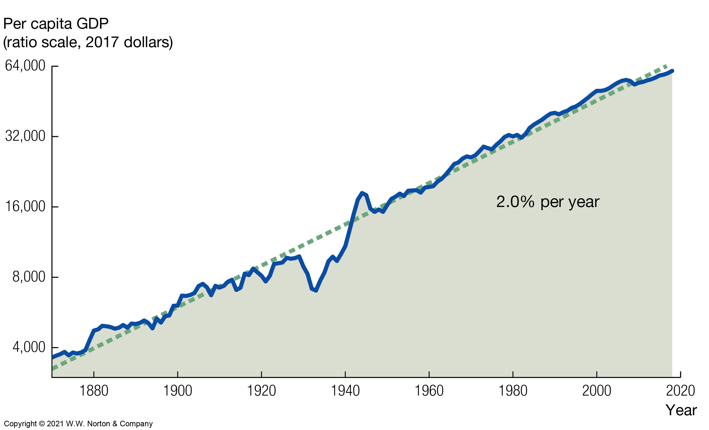
\includegraphics[width=0.7\linewidth]{Figures/ratio_scale}
		\end{figure}
		
	\end{itemize}
\end{frame}

\begin{frame}[wide]{The Ratio (Logarithmic) Scale}
	\begin{itemize}
		\item A plot intervals between tick marks are proportional in terms of ratios rather than absolute differences
		\begin{itemize}
			\item When doubling, we want this constant ratio to be "2." 
			\item e.g., on the y-axis, instead of ``1, 2, 3, 4" we have ''1, 2, 4, 8"
		\end{itemize}
		\item When plotted on a ratio scale, a variable that grows at a constant rate will be a straight line
		\item It is commonly used to represent data where exponential growth or significant variations need to be visually compressed
		\begin{itemize}
			\item Using the population growth figure earlier, we cannot tell right away that the growth rate is constant, increasing, or decreasing
		\end{itemize}
	\end{itemize}
\end{frame}

\begin{frame}[wide]{Population over Time, Revisited}
	\begin{itemize}
		\item Absolute population numbers are increasing faster (left), but the rate of growth is staying the same in the right graph because of the linear relationship (right)
	\end{itemize}
	\begin{figure}
		\centering
		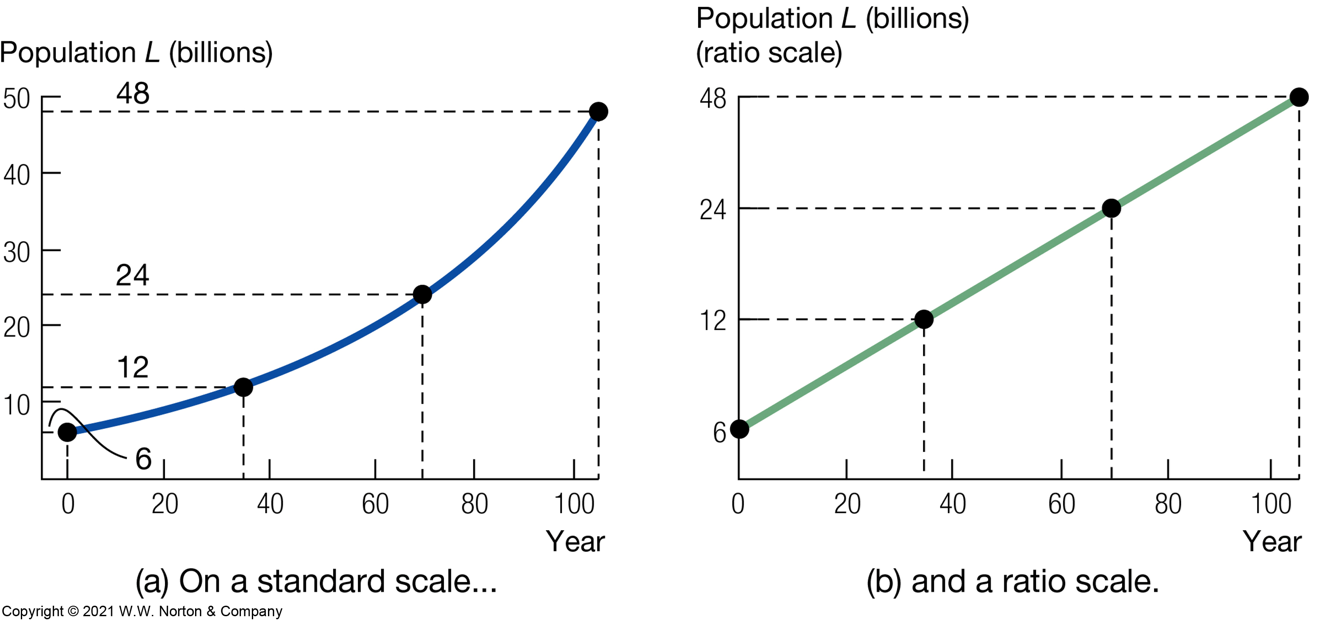
\includegraphics[width=0.7\linewidth]{Figures/ratio_scale1}
	\end{figure}
	
\end{frame}

\begin{frame}[wide]{U.S. GDP on a Ratio Scale}
	\begin{itemize}
		\item On a ratio scale:
		\begin{itemize}
			\item if growth rates are rising, the slope will be increasing
			\item if the growth rate is constant, it will be a straight line
			\item if the growth rate is falling, the slope will be decreasing
		\end{itemize}
		\item Per capita GDP in the United States has grown at approximately 2 percent per year over the past 150 years.
		\begin{itemize}
			\item This outcome is easy to see using a ratio scale
			\item Approximately linear
		\end{itemize}
		
	\end{itemize}
\end{frame}

\begin{frame}[wide]{Per Capita GDP in the United States, Standard vs. Ratio Scale}
	\begin{itemize}
		\item The graph on the left is a standard scale and the one on the right is a ratio scale
		\item Data series lies close to a line that exhibits a constant slope of 2.0 percent per year
		\item To a first approximation, per capita GDP in the United States has been growing at a relatively constant annual rate of 2 percent over the past 150 years
	\end{itemize}
	\begin{figure}
		\centering
		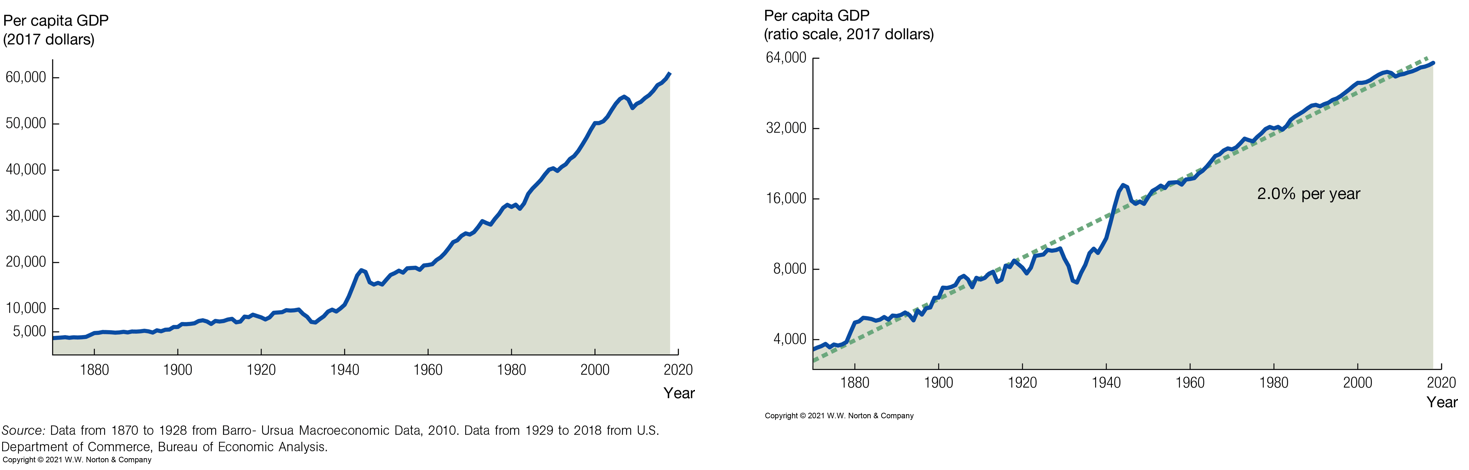
\includegraphics[width=0.8\linewidth]{Figures/US_GDP_ratio_scale}
	\end{figure}
	
\end{frame}

\begin{frame}[wide]{The Ratio Scale in Action: Per Capita GDP since 1870}
	\begin{itemize}
		\item The picture contains more information, but we have to read it carefully
		\item The per capita income line is flag for the UK relative to the US until the 50s
		\item From 1880 to 1920, Argentina grew rapidly; Since 1980, growth has slowed considerably
		\begin{figure}
			\centering
			\includegraphics[width=0.5\linewidth]{"Figures/The Ratio Scale in Action"}
		\end{figure}
	\end{itemize}
\end{frame}

\begin{frame}[wide]{Modern Growth around the World}
	\begin{itemize}
		\item In the late nineteenth century, the United Kingdom was the richest country in the world, but it start grew substantially more slowly than the United States in the 20th century
		\item After World War II, growth in Germany and Japan were similar, in that they both accelerated
		\item Argentina had accelerated growth until 1980 and then slowed considerably
		\item China, Vietnam and India have start ``converging'' recently
		\item \textbf{Convergence}:
		\begin{itemize}
			\item Poorer countries will grow faster to “catch up” to the level of income in richer countries
		\end{itemize}
	\end{itemize}
\end{frame}

\begin{frame}[wide]{A Broad Sample of Countries}
	\begin{itemize}
		\item Over the period 1960--2017:
		\begin{itemize}
			\item Some countries have displayed negative growth rates.
			\item Other countries have maintained growth rates of nearly 7\%.
			\item Most countries have maintained approximately 2\% growth rates.
			\item Small variances in growth rates lead to significant differences in standards of living.
		\end{itemize}
	\end{itemize}
\end{frame}

\begin{frame}[wide]{Levels and Growth Rates of Per Capita GDP}
	\begin{itemize}
		\item From 1960 to 2017, growth rates ranged from -2 percent to +7 percent per year
		\item South Korea, Singapore, Botswana, and Japan grew the fastest over this period
		\item Central African Republic, the Democratic Republic of the Congo, Niger, and Guinea all had negative average growth
		\begin{figure}
			\centering
			\includegraphics[width=0.6\linewidth]{"../Week 4/Figures/Levels and Growth Rates of Per Capita GDP"}
		\end{figure}
		
	\end{itemize}
\end{frame}

\begin{frame}[wide]{Case Study: People versus Countries}
	\begin{itemize}
		\item Compare 2017 to 1960, the bulk of the world’s population is substantially richer and  the fraction of people living in poverty has fallen
		\item A major reason for changes:
		\begin{itemize}
			\item Economic growth in China and India
			\item These two countries account for 40 percent of the world population
		\end{itemize}
	\end{itemize}
	\begin{figure}
		\centering
		\includegraphics[width=0.5\linewidth]{"../Week 4/Figures/People versus Countries"}
	\end{figure}
	
\end{frame}

\begin{frame}[wide]{Some Useful Properties of Growth Rates}
	\begin{itemize}
		\item A lot of time we have economic variables express in term of some mathematical combination of other variables (e.g., GDP per Capita)
		\item Growth rates of ratios, products, and powers follow several (approx.) simple rules
		\item Suppose two variables $x$, $y$ and $z$ have average annual growth rates of $g_x$, $g_y$ and $z$, respectively. Then
		\vspace{1mm}
		\[\text{If } z=x/y \text{, then  } g_z=g_x-g_y\]
		\vspace{1mm}
		\[\text{If } z=x\times y \text{, then  } g_z=g_x+g_y\]
		\vspace{1mm}
		\[\text{If } z=x^a \text{, then  } g_z=a \times g_x\]
		\item We can combine these rules 
	\end{itemize}
\end{frame}

\begin{frame}[wide]{Examples of Growth Rate Calculations}
	\begin{figure}
		\centering
		\includegraphics[width=0.7\linewidth]{"../Week 4/Figures/Examples of Growth Rate"}
	\end{figure}
	
\end{frame}

\begin{frame}[wide]{U.S. Population, GDP, and Per Capita GDP}
	\begin{itemize}
		\item Total GDP = GDP per capita $\times$ number of workers,
		\item Growth rate of total GDP = growth rate of per capita GDP + the growth rate of the population
		\begin{figure}
			\centering
			\includegraphics[width=0.5\linewidth]{"../Week 4/Figures/U.S. Population, GDP, and Per Capita GDP"}
		\end{figure}
		
	\end{itemize}
\end{frame}

\begin{frame}[wide]{Example: Growth Rules with Cobb Douglas Production Function}
	\begin{itemize}
		\item Applying rules of growth rates to a Cobb Douglas production function (see Ch.4):
		\[Y_t = A_t K_t^{1/3} L_t^{2/3}\]
		\item It says the output depends on the levels of technology, capital, and labor. Its growth rate of output can be decomposed into growth rate of a productivity term A,	contributions to growth from capital K, and labor L
		\item Using $\text{If } z=x\times y \text{, then  } g_z=g_x+g_y$,
		\[g(y) = g(A) + g(K^{1/3}) + g(L^{2/3})\]
		\item Then, use $\text{If } z=x^a \text{, then  } g_z=a \times g_x$, 
		\[g(y) = g(A) + \frac{1}{3}g(K) + \frac{2}{3} g(L)\]
	\end{itemize}
\end{frame}

\begin{frame}[wide]{The Benefits and Costs of Economic Growth}
	\begin{itemize}
		\item The benefits of economic growth:
		\begin{itemize}
			\item Improvements in health
			\item Higher incomes
			\item Increase in the variety of goods and services
		\end{itemize}
		\item Costs of economic growth include:
		\begin{itemize}
			\item Environmental problems
			\item Income inequality across and within countries
			\item Loss of certain types of jobs
		\end{itemize}
		\item	Economists generally have a consensus that the benefits of economic growth outweigh the costs.
	\end{itemize}
\end{frame}

\begin{frame}[wide]{What are You Going to Learn (ch. 4)}
	\begin{itemize}
		\item How to set up and solve a macroeconomic model
		\item The purpose of a production function and its use for understanding differences in GDP per capita across countries
		\item The role of capital per person and technology in explaining differences in economic growth
		\item The relevance of “returns to scale” and “diminishing marginal products.”
		\item How to look at economic data through the lens of a macroeconomic model
	\end{itemize}
\end{frame}

\begin{frame}[wide]{Introduction}
	\begin{itemize}
		\item Recalling that a model:
		\begin{itemize}
			\item is a mathematical representation of a hypothetical world that we use to study economic phenomena
			\item consists of equations and unknowns with real-world interpretations
			\begin{itemize}
				\item Mathematically, a model is no more than a set of equations
			\end{itemize}
		\end{itemize}
		\item Economists ...
		\begin{itemize}
			\item Document facts
			\item Build a model to understand the facts
			\item Examine the model to see how effective it is
		\end{itemize}
		
	\end{itemize}
\end{frame}

\begin{frame}[wide]{A Model of Production}
	\begin{itemize}
		\item Even though Model is only a simplifications of the real world, a good model can still  provide important insights
		\item Consider the following model:
		\begin{itemize}
			\item Single, closed economy
			\item One consumption good
		\end{itemize}
		\item Inputs in the production process: Labor ($L$) and Capital ($K$)
		\item Production function: how much output ($Y$) can be produced given any number of inputs		
	\end{itemize}
\end{frame}

\begin{frame}[wide]{Setting Up the Model – Cobb-Douglas  Production Function}
	\[Y=F(K,L) = \bar{A} K^{\alpha}L^{\beta}\]
	\begin{itemize}
		\item The $F$ notation states that \textit{output} ($Y$) is a function of \textit{inputs} ($K$ and $L$) - a general functional form
		\item The production function describes how any amounts of capital and labor can be combined to generate output, not just the particular amount that our toy economy possesses
		\item $\bar{A}$ represents the productivity parameter
		\begin{itemize}
			\item Letters with a bar over them denote parameters that are fixed and exogenously given in the model. These variables stand in for some fixed constant
		\end{itemize}
		\item A higher value of $\bar{A}$ means the firm produces more of the output good with the same amount of inputs
		\begin{itemize}
			\item The bigger the value of the productivity parameter, the more productive the firm.
		\end{itemize}

	\end{itemize}
\end{frame}

\begin{frame}[wide]{Model}
	\[Y=F(K,L) = \bar{A} K^{\alpha}L^{\beta}\]
	\begin{itemize}
		\item Output growth corresponds to changes in $Y$
		\item There are three ways that $Y$ can change:
		\begin{itemize}
			\item Capital stock (K) changes
			\item Labor force (L) changes
			\item Ability to produce goods with given resources (K,L) changes
			\begin{itemize}
				\item Technological advances occur (changes in A)
				\item is assumed to be exogenous in the Solow model (a type of growth model)
			\end{itemize}
		\end{itemize}
	\end{itemize}
\end{frame}

\begin{frame}[wide]{Total Factor Productivity (TFP)}
	\begin{itemize}
		\item Total factor productivity (TFP or Solow residual)
		\item Refers to all inputs that affect output (Y ) except labor and capital
		\item This is the unexplained part of the production function, for example, human capital, energy, land
		\begin{itemize}
			\item It is unexplained in the sense that it is not part of the function or be able to observed directly in the data
		\end{itemize}
		\item An important assumption of the Solow model is that TFP is exogenous
		\item The model makes no effort to explain why TFP equals a particular value
		\begin{itemize}
			\item This is reasonable if we believe that neither policy nor the choices of agents in the model affect its value
			\item However, later we will discuss reasons this is likely a faulty assumption
		\end{itemize}
	\end{itemize}
\end{frame}

\begin{frame}[wide]{More on Cobb-Douglas Production Function}
	\[Y=F(K,L) = \bar{A} K^{\alpha}L^{\beta}\]
	\begin{itemize}
		\item The parameter $\alpha$ and $\beta$ determine the output elasticities of capital and labor
		\item In an usual setup, it also determine the share of labour input and capital output
		\begin{itemize}
			\item The $\alpha$ is usually assume to be 1/3
			\item Recall that the labour income share is roughly 2/3
		\end{itemize}
		\item $F(K,L)$ is increasing in $K$ and $L$
		\begin{itemize}
			\item More inputs yield more output
			\item Formally, $\frac{\partial F}{\partial K} >0 $ and $\frac{\partial F}{\partial L}>0$
		\end{itemize}
	\end{itemize}
\end{frame}

\begin{frame}[wide]{Constant Returns to Scale (CRS)}
	\begin{itemize}
		\item A production function exhibits constant returns to scale if doubling each input exactly doubles output
		\item In the other word, if both $K$ and $L$ increase by $a\%$, then $Y$ also increase by $a\%$
		\item Mathematically,
		\[F(aK,aL) = aF(K,L)\]
		i.e., Homogeneous function (of degree 1)
		\item Usually, we want the production function to be CRS. To do that we restrict the parameter to
		\[\beta = 1-\alpha \text{   and  } 0<\alpha <1\]
		\item The production function became
		\[Y= A K^\alpha L^{1-\alpha}\]
	\end{itemize}
\end{frame}

\begin{frame}[wide]{Constant Returns to Scale (CRS)}
	\begin{itemize}
		\item There are other form of return to scale
		\begin{itemize}
			\item If $\alpha +\beta >1$, the function is increasing return to scale
			\item If $\alpha +\beta =1$, the function is constant return to scale
			\item If $\alpha +\beta <1$, the function is decreasing return to scale
		\end{itemize}
		\item Constant returns to scale guarantee that as you increase the units of labor or capital required to produce your products, you maintain a consistent level of growth (more on that in later chapters)
	\end{itemize}
\end{frame}

\begin{frame}[wide]{Output per Person (Intensive Form)}
	\begin{itemize}
		\item Divide output by the number of workers
		\[\frac{Y}{L} = F\left(\frac{K}{L},\frac{L}{L}\right) = F\left(\frac{K}{L},1\right)\]
		\item In this model, we assume the number of person = number of worker
		\item Lowercase letters denote per capita
		\[y = f(k)\]
		where
		\[y = Y/L\]
		\[k= K/L\]
	\end{itemize}
\end{frame}

\begin{frame}[wide]{Output per Person (Intensive Form)}
	\begin{itemize}
		\item Plot of $y=f(k)=k^{1/3}$, where $y =0$ when $k=0$
		\item Growth models tend to explain deviations in output using changes in K or k
		\item Increasing and features diminishing marginal returns to capital
		\item Production function that is CRS can have diminishing marginal returns in K (or k)
		\begin{figure}
			\centering
			\includegraphics[width=0.45\linewidth]{"Figures/Typical Production Function"}
		\end{figure}
		
	\end{itemize}
\end{frame}

%\begin{frame}[wide]{Measuring the State of the Economy}
%	\begin{columns} 
%		% Column 1
%		\begin{column}{.5\textwidth}
%			\begin{table}[htbp]
%				\centering
%				\begin{tabular}{lrrrr}
%					& 2005  & 2006  & 2007  & 2008 \\
%					\hline
%					GDP   & 12.6  & 13.4  & 14.0    & 14.3 \\
%					(in trillions of \$) &       &       &       &  \\
%					Growth rate GDP &       & 0.063 & 0.045 & 0.021 \\
%					\hline
%				\end{tabular}%
%				\label{tab:addlabel}%
%			\end{table}%
%		\end{column}
%		% Column 2    
%		\begin{column}{.5\textwidth}			
%
%			
%		\end{column}%
%	\end{columns}
%\end{frame}

\begin{frame}[wide]{Next Lecture}
	\begin{itemize}
		\item Next lecture will finish covering Ch.4 
		\item Group assignment will be upload to Crowdmark early next week
		\begin{itemize}
			\item Group up to four students
			\item Once you started, you will have only 3 hours to complete the assignment
			\item Leave enough time for pdf/image upload
		\end{itemize}
	\end{itemize}
\end{frame}

\end{document}